\documentclass[10pt,a4paper]{article}
\usepackage[margin=0.72in]{geometry}
\usepackage{booktabs,graphicx,url,microtype}
\usepackage[T1]{fontenc}
\setlength{\parindent}{1.2em}
\setlength{\parskip}{0.25em}
\title{\vspace{-1.5em}Learning-Augmented Disk Scheduling:\\Adaptive Scheduler Selection Under Workload Shift}
\author{CSE-307 Operating Systems Term Paper}
\date{}
\begin{document}
\maketitle
\vspace{-1.5em}
\begin{abstract}This paper study an adaptive disk scheduler that selects FCFS, SCAN, C-SCAN, or SSTF for each window of 20 requests. A decision tree uses only request statistics available before scheduling. On 450 shared held-out windows, accuracy was 0.858 and mean regret was 4.20 cylinders. The experiment also checks confidence and a sequential-to-random workload shift.\end{abstract}
\section{Problem Framing}
Disk scheduling decide the order in which pending requests are served. For a mechnical disk, the head must move between cylinders, so the chosen order can change total movement. Standard operating systems texts describe FCFS, SSTF, SCAN and C-SCAN as policies with different fairness and movement behavior [1]. This project asks if a learned selector can choose a suitable policy for one re quest window, especially when the request distribution changes.

FCFS follows arrival order. SSTF repeatedly selects the nearest pending cylinder, with the lower cylinder used for an equal-distance tie. SCAN moves to the physical boundary and then reverses. C-SCAN moves in one direction, reaches the boundary, wraps to the other boundary, and continues. Boundary and wrap movement are counted, while total cylinders moved is used as a simple proxy for seek cost.
\section{Classical Algorithms}
FCFS is simple but can make long jumps. SSTF improves locality but may delay distant requests. SCAN gives an elevator-like sweep, and C-SCAN gives a more uniform one-direction service pattern. These definitions follow the conventional presentation of disk scheduling in Operating System Concepts~\cite{silberschatz2018}.
\newpage
\section{Implementation}
The simulator implement all four algorithms from scratch. Three seeded workload generators create sequential, random and bursty traces. Sixteen features describe request location, spread, locality, consecutive jumps, trend, direction changes and entropy. A decision tree was selected because its rules are easy to explain [2], and the implementation uses scikit-learn [3]. The learned s cheduler confidence is the largest predicted class probability.
\section{Experimental Setup}
The disk range was 0-199, initial head was 100, and direction was upward. There was 60 traces for each workload type and 10 windows per trace, giving 1800 windows. The fixed experment seed was 307. Complete traces were kept together: 1350 windows for training and 450 for testing. This avoids putting closely related windows in both groups.

\hspace{0.8em}The same-workload rule was applied directly. Every number in the primary classical and learned comparison is calculated from the exact same held-out windows, request sequences and starting-head positions. These rows are saved in common\_workload\_manifest.csv. Within the shift and generalization tests, all four algorithms and the learned selector also receive the identical window before any cost is compared. No scheduler is given an easier separately generated trace.
\section{Ground Truth and Metrics}
For each shared window, all four classical schedulers are executed from the same head position. The minimum movement is the oracle label. Ties use FCFS, SSTF, SCAN, then C-SCAN. Regret is selected movement minus oracle movement. The decision tree follows the CART family~\cite{breiman1984} and is implemented with scikit-learn~\cite{pedregosa2011}.
\newpage
\section{Results}
The held-out selector accuracy were 0.858. Mean selected movement was 186.22 cylinders per window, compared with 182.02 for the oracle. Mean regret was 4.20. Confidence was 0.945 when correct and 0.887 when wrong. Calibraton ECE was 0.140 and multiclass Brier score was 0.263. Calibration matters because a probability should reflect actual correctness frequency, not only classification accuracy [4].
\begin{table}[h]
\centering\small
\caption{Mean movement on the same held-out windows (lower is better).}
\begin{tabular}{lrrrrrrr}\toprule
Workload & FCFS & SCAN & C-SCAN & SSTF & ML & Oracle & Acc. \\\midrule
Bursty & 264.9 & 213.0 & 300.8 & 123.2 & 123.9 & 123.1 & 0.970 \\
Random & 1332.0 & 283.9 & 381.4 & 256.4 & 244.5 & 240.3 & 0.794 \\
Sequential & 211.5 & 236.5 & 330.4 & 170.5 & 170.0 & 164.0 & 0.853 \\
\bottomrule\end{tabular}
\end{table}
\IfFileExists{../results/figures/classical_scheduler_comparison.png}{\begin{center}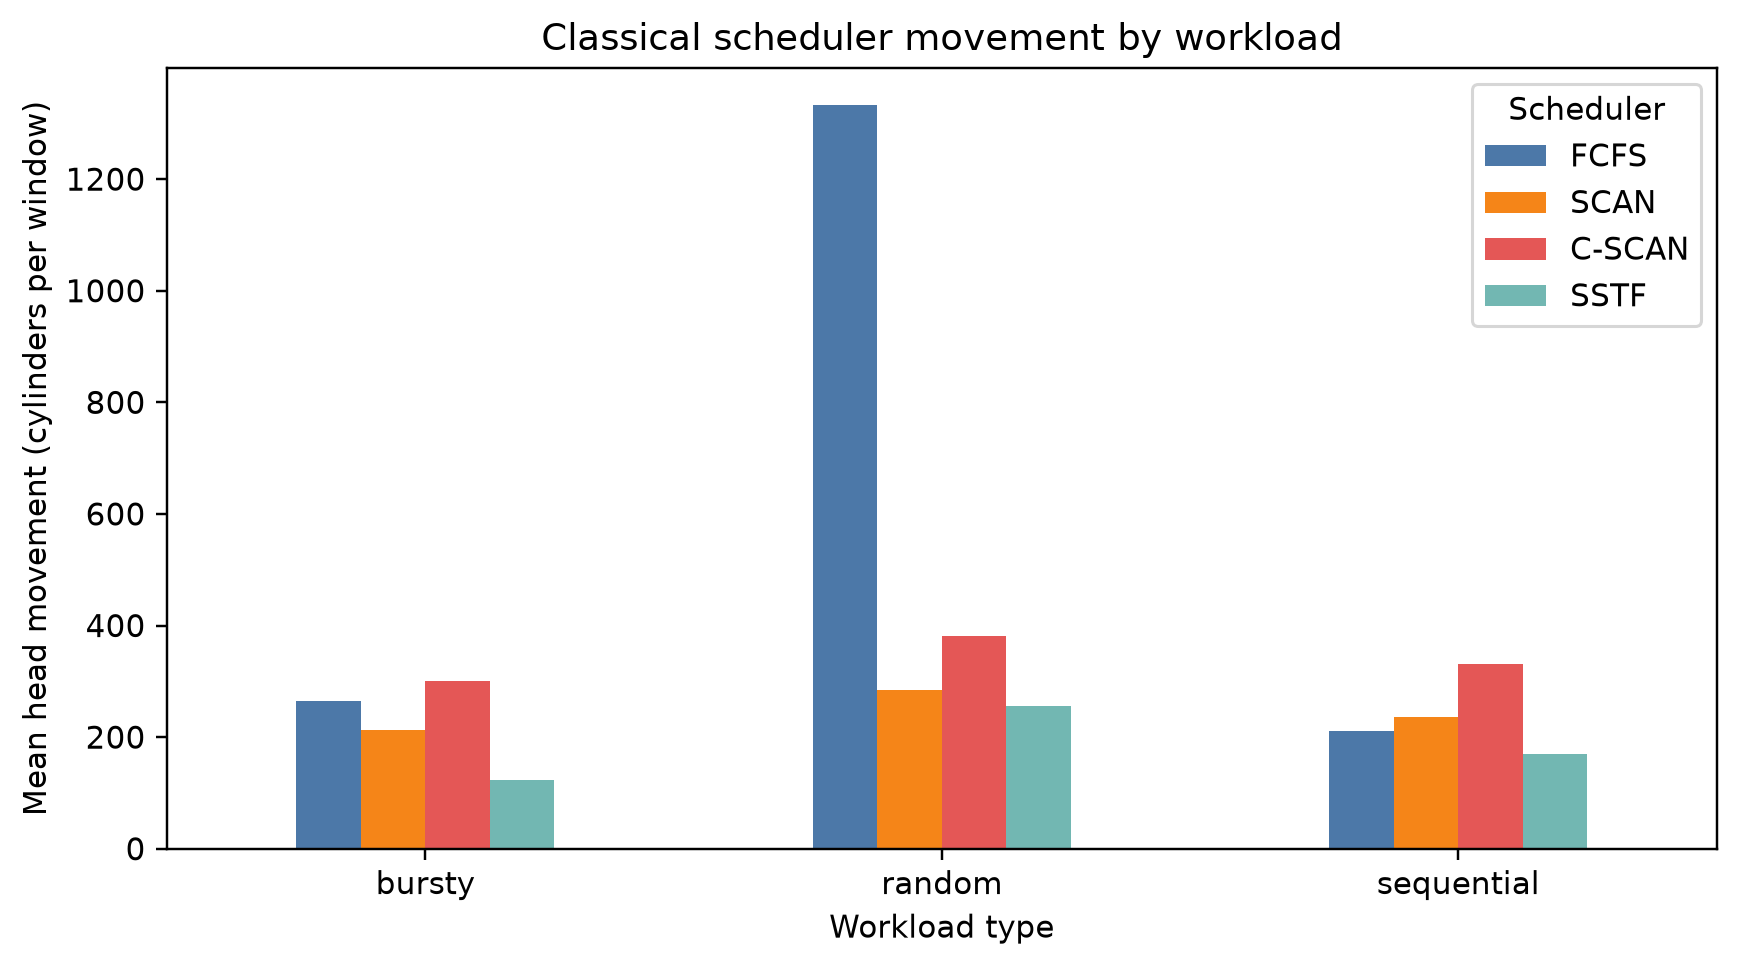
\includegraphics[width=0.75\linewidth]{../results/figures/classical_scheduler_comparison.png}\end{center}}{}
\subsection{Workload Shift}
The shift test use 30 sequential windows followed by 30 random windows. Accuracy changed from 0.933 before the shift to 0.900 after it. Mean movement changed from 159.27 to 196.37, while regret changed from 0.13 to 0.40. The higher movement after the shift mainly reflects the wider random request positions, not a direct causal effect of the classifier.
\begin{table}[h]\centering\small
\begin{tabular}{lrr}\toprule Metric & Before & After \\\midrule
Accuracy & 0.933 & 0.900 \\
Confidence & 0.927 & 0.969 \\
Movement & 159.27 & 196.37 \\
Regret & 0.13 & 0.40 \\\bottomrule
\end{tabular}\end{table}
\newpage
\section{Analysis}
SSTF had the lowest mean movment for bursty, random and sequential windows in the shared test set. This is reasonable because it repeatedly chooses a nearby request. SCAN still provides a structured sweep, while C-SCAN pays a large wrap cost under the selected metric. C-SCAN did not become a true best label in the held-out rows, so its class support was zero. That measured outcome was kept instead of creating artificial favorable cases. The confidence for correct predictions was higher, but the reliability table shows that the tree should not be called perfectly cal ibrated.
\section{Limitations}
The workloads are synthetic and the geometry is a single cylinder line. The simulator does not model request arrival time, rotational delay, caching or real milliseconds. Results therefore describe this classical hard-disk exercise and should not be transferred directly to SSDs. A larger study could use real traces, more seeds and calibrated probability methods.
\section{Conclusion}
The project demonstrates a small learning-augmented scheduler without hiding the cost of wrong choices. Using one common held-out workload makes the fixed-policy and adaptive results directly comparable. The selector came close to the oracle on average, but shift behavior, regret and confidence calibration remain important beside raw classification accuracy.
\section*{AI Assistance Disclosure}
An AI coding assistant was used for software development, testing support, and document drafting. All numerical results were produced by running the included code, and the raw outputs are retained.
\begin{thebibliography}{9}
\bibitem{silberschatz2018} A. Silberschatz, P. B. Galvin, and G. Gagne, \emph{Operating System Concepts}, 10th ed. Wiley, 2018. \url{https://os-book.com/OS10/}
\bibitem{breiman1984} L. Breiman, J. H. Friedman, R. A. Olshen, and C. J. Stone, \emph{Classification and Regression Trees}. Wadsworth \& Brooks/Cole, 1984.
\bibitem{pedregosa2011} F. Pedregosa et al., ``Scikit-learn: Machine Learning in Python,'' \emph{Journal of Machine Learning Research}, vol. 12, pp. 2825--2830, 2011.
\bibitem{guo2017} C. Guo, G. Pleiss, Y. Sun, and K. Q. Weinberger, ``On Calibration of Modern Neural Networks,'' \emph{Proceedings of Machine Learning Research}, vol. 70, pp. 1321--1330, 2017.
\end{thebibliography}
\end{document}
